\documentclass[letter, 10pt]{article}
\usepackage{fullpage}
\usepackage[margin=0.2in]{geometry}
\usepackage{graphicx}
\usepackage{caption}
\usepackage{subcaption}
\usepackage[table]{xcolor}
\usepackage{amsmath}
\usepackage{listings}
\usepackage{float}
\usepackage{array,multirow}
\usepackage{tikz}
\usepackage{cancel}
\usepackage{listings}
\setcounter{MaxMatrixCols}{20}
\usetikzlibrary{arrows}
\pagenumbering{gobble}
\begin{document}
\noindent
\large \textbf{Rahul Ghosh} \hfill \textbf{Assignment\#4}\\
\normalsize Student ID: 5476965 \hfill CSci 5512\\

\section*{Question 1}
\begin{itemize}
    \item[(1)] Pay of Job A lies in $\mathcal{N}(0,1)$ and the pay of job B lies in $\mathcal{N}(0.5,0.5)$. The distribution of both the pays are shown below.

    To be stochastically dominant, the area under Job A should be more than the area under Job B at all times. The total area under the curve for a normal distribution is 1. The area within 3 standard deviation is 99.6\% of the total.
    
    Even though initially the area under the curve of Job A is greater than the area under Job B, Job B has 99.6\% of its area within 2, whereas Job B has 99.6\% of its area within 3. Thus Job B does not stochastically dominate Job A. The plots of both the distribution is shown in Fig1.
    
    \begin{figure}[H]
        \centering
        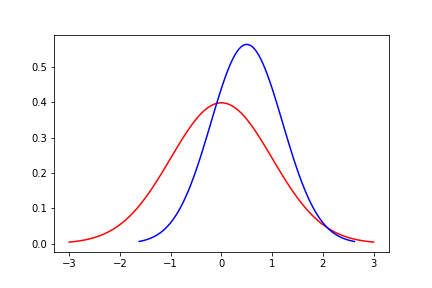
\includegraphics[width=\textwidth, height=0.5\textwidth]{HW4/P1.png}
        \caption{Distribution of Job A and Job B}
    \end{figure}
    
    \item[(2)] For Job Y to stochastically dominate Job X, $\mu_x<\mu_y$ and $\sigma^2_x<\sigma^2_y$.
    
    \item[(3)] The AUC of normal distribution is 0 at $-\infty$ and becomes 1 at $\infty$. Whereas, the AUC of uniform distribution U(a,b) becomes greater than zero at a and becomes 1 at b. Therefore the normal distribution will always have more area initially and the uniform distribution will always reach area=1 before. So, neither uniform distribution stochastically dominates uniform distribution nor vice versa.
\end{itemize}

\newpage

\section*{Question 2}
Since initially we don't know the machine, therefore all the machines are equally likely.
\begin{itemize}
    \item SLOT(X) $\rightarrow$ U(X) = $\frac{10}{100}\times20+\frac{30}{100}\times5+\frac{40}{100}\times1+\frac{20}{100}\times0 = 2+1.5+0.4+0 = 3.9$
    \item SLOT(Y) $\rightarrow$ U(Y) = $\frac{5}{100}\times40+\frac{25}{100}\times4+\frac{30}{100}\times2+\frac{40}{100}\times0 = 2+1+0.6+0 = 3.6$
    \item SLOT(Z) $\rightarrow$ U(Z) = $\frac{25}{100}\times10+\frac{25}{100}\times5+\frac{25}{100}\times2+\frac{25}{100}\times0 = 2.5+1.25+0.5+0 = 4.25$
\end{itemize}
$\implies U(X or Y or Z) = \frac{1}{3}\times3.9+\frac{1}{3}\times3.6+\frac{1}{3}\times4.25 = \frac{11.75}{3}$\\

Now, identifying one of the slot machines will give rise to three cases:
\begin{itemize}
    \item[1.] SLOT(X) is identified.\\
    $\implies U(Y or Z) = \frac{3.6 + 4.25}{2} = \frac{7.85}{2} = 3.925$\\
    Since $U(Y or Z)>U(X)$, the best action would be to play on the remaining two machines.
    \item[2.] SLOT(Y) is identified.\\
    $\implies U(X or Z) = \frac{3.9 + 4.25}{2} = \frac{8.15}{2} = 4.075$\\
    Since $U(X or Z)>U(Y)$, the best action would be to play on the remaining two machines.
    \item[2.] SLOT(Z) is identified.\\
    $\implies U(X or Y) = \frac{3.9 + 3.6}{2} = \frac{7.5}{2} = 3.75$\\
    Since $U(Z)>U(XorY)$, the best action would be to play on the identified Z machine.
\end{itemize}

Each of the aboe cases have equal probability of happening. Therefore the utility of getting one of the slot machine identified is,\\
$\implies U = \frac{1}{3}\times3.925+\frac{1}{3}\times4.075+\frac{1}{3}\times4.25 = \frac{12.25}{3}$\\

Difference in Utility = $U-U(X or Y or Z) = \frac{12.25}{3}-\frac{11.75}{3} = \frac{0.5}{3} = 0.166667$

Therefore, we should be willing to pay 0.166667\$ to get the identification done.

\section*{Question 3}
\begin{equation*}
    Reward(s) = \begin{tabular}{ |c|c|c| } 
                \hline
                \cellcolor{black}coloured & 50 & \cellcolor{black}coloured\\
                \hline
                \cellcolor{black}coloured & 0 & -3\\
                \hline
                -50 & -1 & -10\\
                \hline
                \cellcolor{black}coloured & -3 & -2\\
                \hline
                \end{tabular}\quad
    \gamma = 0.8\quad
    Probability(a) = \{0.7, 0.15, 0.15\}
\end{equation*}
\begin{itemize}
    \item[(1)] \begin{equation*}
                    Initial State = \begin{tabular}{ |c|c|c| } 
                                    \hline
                                    \cellcolor{black}coloured & 50 & \cellcolor{black}coloured\\
                                    \hline
                                    \cellcolor{black}coloured & 4 & 8\\
                                    \hline
                                    -50 & 7 & 4\\
                                    \hline
                                    \cellcolor{black}coloured & 9 & 5\\
                                    \hline
                                    \end{tabular}\quad 
                    Final State =   \begin{tabular}{ |c|c|c| } 
                                    \hline
                                    \cellcolor{black}coloured & 50 & \cellcolor{black}coloured\\
                                    \hline
                                    \cellcolor{black}coloured & 33.87 & 17.3\\
                                    \hline
                                    -50 & 11.43 & -0.38\\
                                    \hline
                                    \cellcolor{black}coloured & 2.70 & -1.18\\
                                    \hline
                                    \end{tabular}
                \end{equation*}
                \begin{equation*}
                    Initial Policy = \begin{tabular}{ |c|c|c| } 
                                    \hline
                                    \cellcolor{black}coloured & 50 & \cellcolor{black}coloured\\
                                    \hline
                                    \cellcolor{black}coloured & $\uparrow$ & $\uparrow$\\
                                    \hline
                                    -50 & $\rightarrow$ & $\leftarrow$\\
                                    \hline
                                    \cellcolor{black}coloured & $\rightarrow$ & $\rightarrow$\\
                                    \hline
                                    \end{tabular}\quad 
                    Final Policy =   \begin{tabular}{ |c|c|c| } 
                                    \hline
                                    \cellcolor{black}coloured & 50 & \cellcolor{black}coloured\\
                                    \hline
                                    \cellcolor{black}coloured & $\uparrow$ & $\leftarrow$\\
                                    \hline
                                    -50 & $\uparrow$ & $\uparrow$\\
                                    \hline
                                    \cellcolor{black}coloured & $\uparrow$ & $\leftarrow$\\
                                    \hline
                                    \end{tabular}
                \end{equation*}
                \begin{equation*}
                    Num\_Iterations = 4
                \end{equation*}
    \item[(2)] \begin{equation*}
                    Initial State = \begin{tabular}{ |c|c|c| } 
                                    \hline
                                    \cellcolor{black}coloured & 50 & \cellcolor{black}coloured\\
                                    \hline
                                    \cellcolor{black}coloured & 0 & 0\\
                                    \hline
                                    -50 & 0 & 0\\
                                    \hline
                                    \cellcolor{black}coloured & 0 & 0\\
                                    \hline
                                    \end{tabular}\quad 
                    Final State =   \begin{tabular}{ |c|c|c| } 
                                    \hline
                                    \cellcolor{black}coloured & 50 & \cellcolor{black}coloured\\
                                    \hline
                                    \cellcolor{black}coloured & 33.68 & 16.72\\
                                    \hline
                                    -50 & 11.04 & -1.38\\
                                    \hline
                                    \cellcolor{black}coloured & 1.47 & -2.97\\
                                    \hline
                                    \end{tabular}
                \end{equation*}
                \begin{equation*}
                    Initial Policy = \begin{tabular}{ |c|c|c| } 
                                    \hline
                                    \cellcolor{black}coloured & 50 & \cellcolor{black}coloured\\
                                    \hline
                                    \cellcolor{black}coloured & $\uparrow$ & $\uparrow$\\
                                    \hline
                                    -50 & $\rightarrow$ & $\leftarrow$\\
                                    \hline
                                    \cellcolor{black}coloured & $\uparrow$ & $\uparrow$\\
                                    \hline
                                    \end{tabular}\quad 
                    Final Policy =   \begin{tabular}{ |c|c|c| } 
                                    \hline
                                    \cellcolor{black}coloured & 50 & \cellcolor{black}coloured\\
                                    \hline
                                    \cellcolor{black}coloured & $\uparrow$ & $\leftarrow$\\
                                    \hline
                                    -50 & $\uparrow$ & $\uparrow$\\
                                    \hline
                                    \cellcolor{black}coloured & $\uparrow$ & $\leftarrow$\\
                                    \hline
                                    \end{tabular}
                \end{equation*}
                \begin{equation*}
                    Num\_Iterations = 4
                \end{equation*}
    \item[(3)] From (1) and (2) we have two sets of utilities. When we use Bellman's equations, then for every update we have
    \begin{equation}
        \left\|U_0-U_0'\right\|\geq\gamma\left\|U_1-U_1'\right\|
    \end{equation}
    In this question, let $\left\|U_0-U_0'\right\| = \sum_{cell}(U_0[cell]-U_0'[cell])$.\\
    Thus the difference in utility at every iteration is [37, 30.04, 17.51, 10.21, 5.20].\\
    Figure 2 shows the plot of $\left\|U_0-U_0'\right\|\ and \ \gamma\left\|U_1-U_1'\right\|$
    \begin{figure}[H]
        \centering
        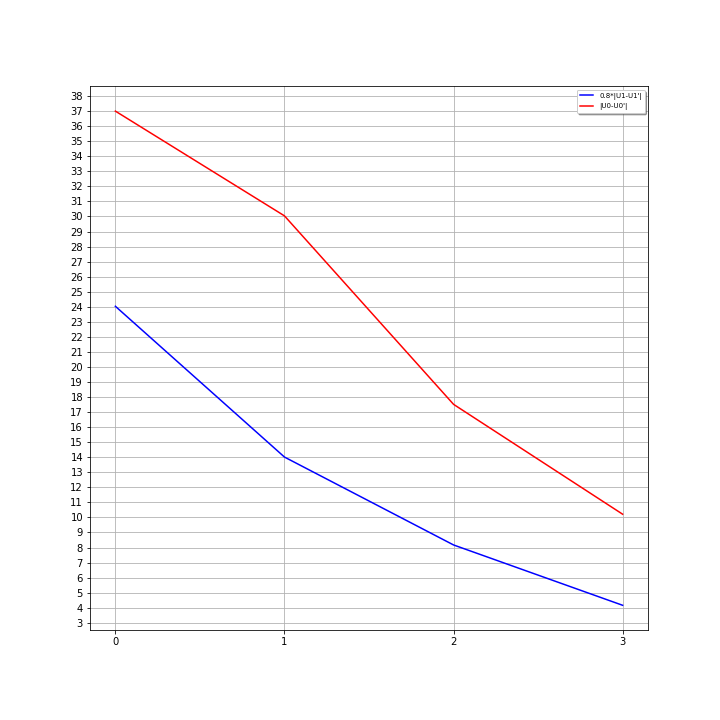
\includegraphics[width=\textwidth, height=\textwidth]{HW4/P3.png}
        \caption{$\left\|U_0-U_0'\right\|\ and \ \gamma\left\|U_1-U_1'\right\|$}
    \end{figure}
\end{itemize}
\newpage

\section*{Question 4}
\begin{equation*}
    Initial Policy = \begin{tabular}{ |c|c|c| } 
                    \hline
                    \cellcolor{black}coloured & 50 & \cellcolor{black}coloured\\
                    \hline
                    \cellcolor{black}coloured & $\uparrow$ & $\uparrow$\\
                    \hline
                    -50 & $\uparrow$ & $\uparrow$\\
                    \hline
                    \cellcolor{black}coloured & $\uparrow$ & $\uparrow$\\
                    \hline
                    \end{tabular}\quad
\end{equation*}
$U(0,1) = 50\\
U(1,1) = -1 + 0.8(0.7\times U(0,1) + 0.15 \times U(1,1) + 0.15 \times U(1,2))\\
U(1,2) = -1 + 0.8(0.7\times U(1,2) + 0.15 \times U(1,1) + 0.15 \times U(1,2))\\
U(2,0) = -50\\
U(2,1) = -1 + 0.8(0.7\times U(1,1) + 0.15 \times U(2,0) + 0.15 \times U(2,2))\\
U(2,2) = -1 + 0.8(0.7\times U(1,2) + 0.15 \times U(2,1) + 0.15 \times U(2,2))\\
U(3,1) = -1 + 0.8(0.7\times U(2,1) + 0.15 \times U(3,1) + 0.15 \times U(3,2))\\
U(3,2) = -1 + 0.8(0.7\times U(2,2) + 0.15 \times U(3,1) + 0.15 \times U(3,2))\\
$
Solving this system of linewar equations we get the value of utilities for each cell.
\begin{equation*}
    Utility = \begin{tabular}{ |c|c|c| } 
                \hline
                \cellcolor{black}coloured & 50 & \cellcolor{black}coloured\\
                \hline
                \cellcolor{black}coloured & 34.38 & 18.78\\
                \hline
                -50 & 12.53 & 2.29\\
                \hline
                \cellcolor{black}coloured & 4.70 & 1.03\\
                \hline
                \end{tabular}
\end{equation*}
Then we again get the best policy for these utilities and repeat until the policies converge.

The change in policies and utilities in every iteration are given below.
\begin{equation*}
    \begin{tabular}{ |c|c|c| } 
    \hline
    \cellcolor{black}coloured & 50 & \cellcolor{black}coloured\\
    \hline
    \cellcolor{black}coloured & $\uparrow$ & $\uparrow$\\
    \hline
    -50 & $\uparrow$ & $\uparrow$\\
    \hline
    \cellcolor{black}coloured & $\uparrow$ & $\uparrow$\\
    \hline
    \end{tabular}\rightarrow
    \begin{tabular}{ |c|c|c| } 
    \hline
    \cellcolor{black}coloured & 50 & \cellcolor{black}coloured\\
    \hline
    \cellcolor{black}coloured & $\uparrow$ & $\leftarrow$\\
    \hline
    -50 & $\uparrow$ & $\leftarrow$\\
    \hline
    \cellcolor{black}coloured & $\uparrow$ & $\leftarrow$\\
    \hline
    \end{tabular}\rightarrow
    \begin{tabular}{ |c|c|c| } 
    \hline
    \cellcolor{black}coloured & 50 & \cellcolor{black}coloured\\
    \hline
    \cellcolor{black}coloured & $\uparrow$ & $\leftarrow$\\
    \hline
    -50 & $\uparrow$ & $\uparrow$\\
    \hline
    \cellcolor{black}coloured & $\uparrow$ & $\leftarrow$\\
    \hline
    \end{tabular}
\end{equation*}

\begin{equation*}
    \begin{tabular}{ |c|c|c| } 
    \hline
    \cellcolor{black}coloured & 50 & \cellcolor{black}coloured\\
    \hline
    \cellcolor{black}coloured & 32.19 & 2.69\\
    \hline
    -50 & 10.30 & -8.28\\
    \hline
    \cellcolor{black}coloured & 1.982 & -7.27\\
    \hline
    \end{tabular}\rightarrow
    \begin{tabular}{ |c|c|c| } 
    \hline
    \cellcolor{black}coloured & 50 & \cellcolor{black}coloured\\
    \hline
    \cellcolor{black}coloured & 34.31 & 18.29\\
    \hline
    -50 & 12.096 & -0.988\\
    \hline
    \cellcolor{black}coloured & 4.336 & 0.352\\
    \hline
    \end{tabular}\rightarrow
    \begin{tabular}{ |c|c|c| } 
    \hline
    \cellcolor{black}coloured & 50 & \cellcolor{black}coloured\\
    \hline
    \cellcolor{black}coloured & 34.38 & 18.78\\
    \hline
    -50 & 12.53 & 2.29\\
    \hline
    \cellcolor{black}coloured & 4.70 & 1.03\\
    \hline
    \end{tabular}
\end{equation*}

\begin{equation*}
    Final Policy =   \begin{tabular}{ |c|c|c| } 
                    \hline
                    \cellcolor{black}coloured & 50 & \cellcolor{black}coloured\\
                    \hline
                    \cellcolor{black}coloured & $\uparrow$ & $\leftarrow$\\
                    \hline
                    -50 & $\uparrow$ & $\uparrow$\\
                    \hline
                    \cellcolor{black}coloured & $\uparrow$ & $\leftarrow$\\
                    \hline
                    \end{tabular}
    Final Utility = \begin{tabular}{ |c|c|c| } 
                    \hline
                    \cellcolor{black}coloured & 50 & \cellcolor{black}coloured\\
                    \hline
                    \cellcolor{black}coloured & 34.38 & 18.78\\
                    \hline
                    -50 & 12.53 & 2.29\\
                    \hline
                    \cellcolor{black}coloured & 4.70 & 1.03\\
                    \hline
                    \end{tabular}\quad Num\_Iterations = 3
\end{equation*}

The code for the above calulations is shown in the next page.
\newpage
\begin{lstlisting}[language=Python]
#!/usr/bin/env python3
# -*- coding: utf-8 -*-
"""
Created on Mon Apr  8 10:54:39 2019

@author: ghosh128
"""

#MDP
import copy
import numpy as np

ACTIONS = []
ACTIONS.append([-1, 0])
ACTIONS.append([1, 0])
ACTIONS.append([0, -1])
ACTIONS.append([0, 1])

rows = 4
columns = 3
reward = [[None, 50, None],
          [None, 0, -3],
          [-50, -1, -10],
          [None, -3, -2]]
terminal_states = [[0, 1], [2, 0]]
state = [[None, 50, None], [None, 0, 0], [-50, 0, 0], [None, 0, 0]]
policy = [[None, 50, None],
          [None, ACTIONS[0], ACTIONS[0]],
          [-50, ACTIONS[0], ACTIONS[0]],
          [None, ACTIONS[0], ACTIONS[0]]]
probability = [0.7, 0.15, 0.15]
gamma = 0.8
index_list = [[0,1], [1,1], [1,2], [2,0], [2,1], [2,2], [3,1], [3,2]]

def action_list(action):
    if not action[1]:
        return [action, [0, -1], [0, 1]]
    else:
        return [action, [-1, 0], [1, 0]]

def apply_action(action, i, j):
    actions = action_list(action)
    value = 0
    for step,action in enumerate(actions):
        new_i = i+action[0]
        new_j = j+action[1]
        if new_i<0 or new_i>=rows or new_j<0 or new_j>=columns or reward[new_i][new_j] is None:
            new_i = i
            new_j = j
        value += probability[step]*state[new_i][new_j]
    return value

def get_equation(i, j):
    a = np.zeros(len(index_list))
    b = reward[i][j]
    a[index_list.index([i, j])] = 1
    if [i, j] in terminal_states:
        return a, b
    else:
        actions = action_list(policy[i][j])
        for step, action in enumerate(actions):
            new_i = i+action[0]
            new_j = j+action[1]
            if new_i<0 or new_i>=rows or new_j<0 or new_j>=columns or reward[new_i][new_j] is None:
                new_i = i
                new_j = j
            a[index_list.index([new_i, new_j])] += (-1*gamma*probability[step])
        return a, b
    
def get_best_action(i,j):
    value_up = apply_action(ACTIONS[0], i, j)
    value_down = apply_action(ACTIONS[1], i, j)
    value_left = apply_action(ACTIONS[2], i, j)
    value_right = apply_action(ACTIONS[3], i, j)
    return np.argmax([value_up, value_down, value_left, value_right])

state_all = []
policy_all = []
iter = 0
count = len(index_list)
while count != 0:
    policy_all.append(copy.deepcopy(policy))
    A = np.zeros(len(index_list))
    B = []
    for index in index_list:
        a, b = get_equation(index[0], index[1])
        A = np.vstack((A, np.reshape(a, (1,-1))))
        B.append(b)
    A = A[1:,:]
    x = np.linalg.solve(A, B)

    for i, index in enumerate(index_list):
        if index not in terminal_states:
            state[index[0]][index[1]] = x[i]
    
    state_all.append(copy.deepcopy(state))
    new_policy = copy.deepcopy(policy)
    count=0
    for i, index in enumerate(index_list):
        if index not in terminal_states:
            new_policy[index[0]][index[1]] = ACTIONS[get_best_action(index[0], index[1])]
            if new_policy[index[0]][index[1]][0] is not policy[index[0]][index[1]][0] or 
            new_policy[index[0]][index[1]][1] is not policy[index[0]][index[1]][1]:
                print(new_policy[index[0]][index[1]], policy[index[0]][index[1]])
                count += 1
    policy = copy.deepcopy(new_policy)
    iter += 1
    print(iter, count)
\end{lstlisting}
\newpage

\section*{Question 5}
Let,
$b(s) = \begin{tabular}{ |c|c| } 
                    \hline
                    a & b\\
                    \hline
                    c & d\\
                    \hline
                \end{tabular},\quad
Probability(a) = \{0.7, 0.15, 0.15\}\quad
P(e|s) = \begin{tabular}{ |c|c| } 
            \hline
            0.3 & 0\\
            \hline
            0.9 & 0.2\\
            \hline
        \end{tabular}\quad
b(s') = \begin{tabular}{ |c|c| } 
            \hline
            A & B\\
            \hline
            C & D\\
            \hline
        \end{tabular}$
\\

Suppose the chosen action is "LEFT". Then,\\
$
A = 0.3\times (0.85\times a + 0.7\times b + 0.15\times c + 0\times d)\\
B = 0\times (0\times a + 0.15\times b + 0\times c + 0.15\times d)\\
C = 0.9\times (0.15\times a + 0\times b + 0.85\times c + 0.7\times d)\\
D = 0.2\times (0\times a + 0.15\times b + 0\times c + 0.15\times d)\\
$

Similarly if the chosen action is "DOWN". Then,\\
$
A = 0.3\times (0.15\times a + 0.15\times b + 0\times c + 0\times d)\\
B = 0\times (0.15\times a + 0.15\times b + 0\times c + 0\times d)\\
C = 0.9\times (0.7\times a + 0\times b + 0.85\times c + 0.15\times d)\\
D = 0.2\times(0\times a + 0.7\times b + 0.15\times c + 0.85\times d)
$
\\

R(s) = $c - a - 4\times b - 2\times d$\\
The sequence of actions for this problem can be
\begin{itemize}
    \item[1] LEFT, DOWN
    $\implies   \begin{tabular}{ |c|c| } 
                    \hline
                    0.2 & 0.3\\
                    \hline
                    0 & 0.5\\
                    \hline
                \end{tabular} \xrightarrow{\text{LEFT}}
                \begin{tabular}{ |c|c| } 
                    \hline
                    0.114 & 0\\
                    \hline
                    0.342 & 0.0024\\
                    \hline
                \end{tabular} \xrightarrow{\text{DOWN}}
                \begin{tabular}{ |c|c| } 
                    \hline
                    0.00513 & 0\\
                    \hline
                    0.33669 & 0.01434\\
                    \hline
                \end{tabular}\implies$
    REWARD = 0.30288
    \item[2] LEFT, LEFT
    $\implies   \begin{tabular}{ |c|c| } 
                    \hline
                    0.2 & 0.3\\
                    \hline
                    0 & 0.5\\
                    \hline
                \end{tabular} \xrightarrow{\text{LEFT}}
                \begin{tabular}{ |c|c| } 
                    \hline
                    0.114 & 0\\
                    \hline
                    0.342 & 0.0024\\
                    \hline
                \end{tabular} \xrightarrow{\text{LEFT}}
                \begin{tabular}{ |c|c| } 
                    \hline
                    0.04446 & 0\\
                    \hline
                    0.29214 & 0.00072\\
                    \hline
                \end{tabular}\implies$
    REWARD = 0.24624
    \item[3] DOWN, LEFT
    $\implies   \begin{tabular}{ |c|c| } 
                    \hline
                    0.2 & 0.3\\
                    \hline
                    0 & 0.5\\
                    \hline
                \end{tabular} \xrightarrow{\text{DOWN}}
                \begin{tabular}{ |c|c| } 
                    \hline
                    0.0225 & 0\\
                    \hline
                    0.1935 & 0.127\\
                    \hline
                \end{tabular} \xrightarrow{\text{LEFT}}
                \begin{tabular}{ |c|c| } 
                    \hline
                    0.014445 & 0\\
                    \hline
                    0.231075 & 0.00381\\
                    \hline
                \end{tabular}\implies$
    REWARD = 0.20901
    \item[4] DOWN, DOWN
    $\implies   \begin{tabular}{ |c|c| } 
                    \hline
                    0.2 & 0.3\\
                    \hline
                    0 & 0.5\\
                    \hline
                \end{tabular} \xrightarrow{\text{DOWN}}
                \begin{tabular}{ |c|c| } 
                    \hline
                    0.0225 & 0\\
                    \hline
                    0.1935 & 0.127\\
                    \hline
                \end{tabular} \xrightarrow{\text{DOWN}}
                \begin{tabular}{ |c|c| } 
                    \hline
                    0.00101 & 0\\
                    \hline
                    0.17935 & 0.0274\\
                    \hline
                \end{tabular}\implies$
    REWARD = 0.123545
\end{itemize}
Thus, \{LEFT, DOWN\} is the best sequence of actions that can be taken.
\end{document}